\subsection{Design of Symmetric-key Algorithms}

\renewcommand{\TITLE}{\it Design of Symmetric-key Algorithms}

\begin{frame}
\CurTitle{}

\vspace{1.25cm}

\Center{
    \large \textit{Lightweight} Cryptography:

    \vspace{0.25cm}

    \large Cryptography for \textcolor{red}{resource-constrained} devices \\
    (Internet of Things)
}
\end{frame}


\begin{frame}[t]
\CurTitle{}

\Center{
\hspace*{-1cm}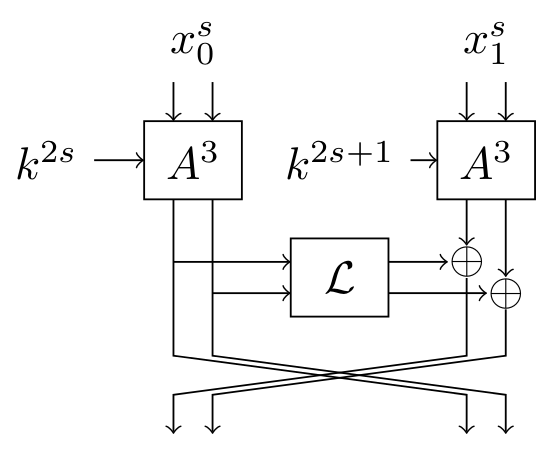
\includegraphics[height=5cm]{figures/Sparx-64-round-function.png}
}

\Center{
    \large \textbf{Sparx}: a \textit{lightweight} block cipher \\
    based on a \textcolor{red}{new design strategy}
}
\end{frame}


\begin{frame}[t]
\CurTitle{}

\Center{
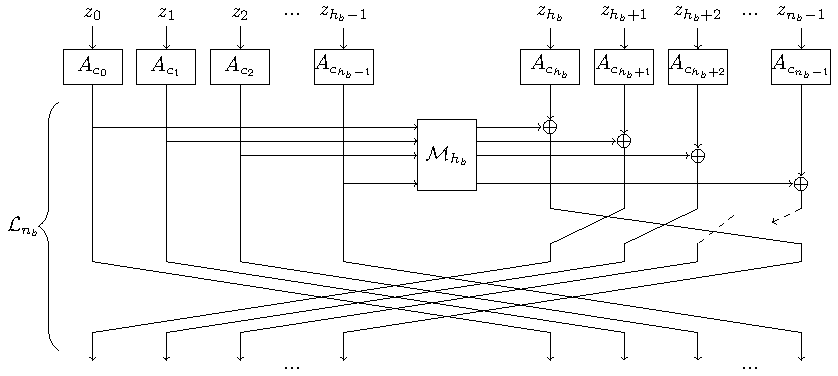
\includegraphics[height=5cm]{figures/step.pdf}
}

\Center{
    \large \textbf{Sparkle}, \textbf{Esch} and \textbf{Schwaemm}:
    
    cryptographic permutations, hash functions \\
    and authenticated encryption
}
\end{frame}


\begin{frame}
    % \begin{center}\Large Part IV. Publications\end{center}
    \begin{center}\Large \TITLE\end{center}
    
    \nocitepartiv{mybibSPARX}
    \nocitepartiv{mybibSPARKLE}
    \bibliographystylepartiv{unsrt}
    \bibliographypartiv{mybiblio.bib}
\end{frame}